\subsection{RAID 10}

RAID 1+0 (RAID 10) es un RAID compuesto que combina mirroring (RAID 1) y striping (RAID 0).

Conceptualmente, primero se crean pares de discos en RAID 1, de manera que cada disco tiene un espejo. Luego, esos pares se combinan mediante RAID 0, distribuyendo los datos entre los distintos espejos.

Por ejemplo, un arreglo RAID 10 con cuatro discos tendría una configuración como la representada en la figura \ref{fig:raid10}.

\begin{figure}[!ht]
  \centering
  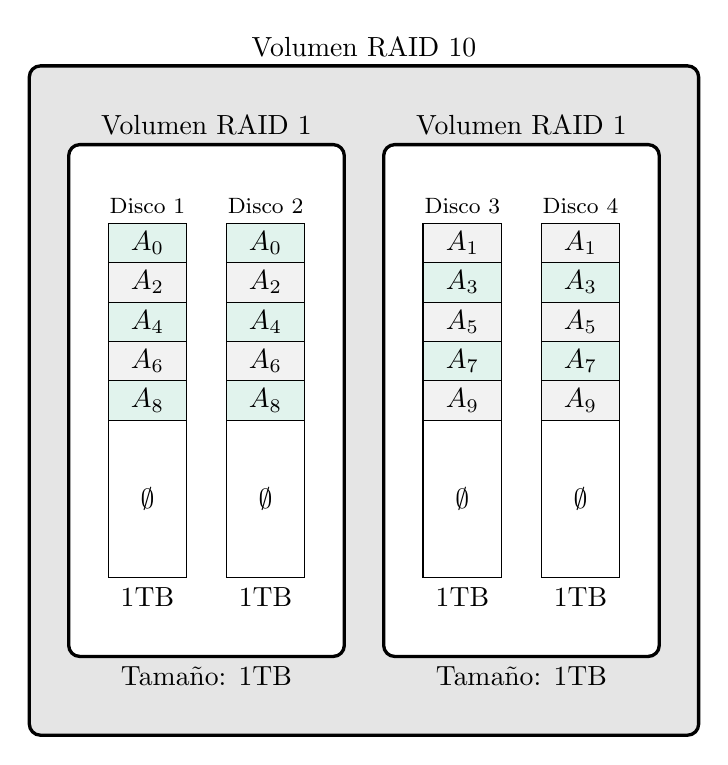
\begin{tikzpicture}
    % RAID 0 

    \draw[very thick,rounded corners,fill=gray!20] (-1,-4) rectangle (7.5,4.5);
    \node[above] at (3.25,4.5) {Volumen RAID 10};

    % caja RAID 1 arreglo 1
    \draw[very thick,rounded corners,fill=white] (-0.5,-3) rectangle (3,3.5);
    \node[above] at (1.25,3.5) {Volumen RAID 1};
    \node[below] at (1.25,-3) {Tamaño: 1TB};

    % caja RAID 1 arreglo 2
    \draw[very thick,rounded corners,fill=white] (3.5,-3) rectangle (7,3.5);
    \node[above] at (5.25,3.5) {Volumen RAID 1};
    \node[below] at (5.25,-3) {Tamaño: 1TB};

    % Primer arreglo de RAID 1

    \node[above,font=\footnotesize] at (0.5,2.5) {Disco 1};
    \foreach \y\t\c in {
        0/8/white!95!blue!93!green,
        0.5/6/gray!10,
        1/4/white!95!blue!93!green,
        1.5/2/gray!10,
        2/0/white!95!blue!93!green}{
      \draw[fill=\c] (0,\y) rectangle node{\(A_\t\)} (1,{0.5+\y});
    }
    \draw (0,0) rectangle node{\(\emptyset\)} (1,-2);
    \node[below] at (0.5,-2) {1TB};

    \node[above,font=\footnotesize] at (2,2.5) {Disco 2};
    \foreach \y\t\c in {
        0/8/white!95!blue!93!green,
        0.5/6/gray!10,
        1/4/white!95!blue!93!green,
        1.5/2/gray!10,
        2/0/white!95!blue!93!green}{
      \draw[fill=\c] (1.5,\y) rectangle node{\(A_\t\)} (2.5,{0.5+\y});
    }
    \draw (1.5,0) rectangle node{\(\emptyset\)} (2.5,-2);
    \node[below] at (2,-2) {1TB};

    % Segundo arreglo de RAID 1

    \node[above,font=\footnotesize] at (4.5,2.5) {Disco 3};
    \foreach \y\t\c in {
        0/9/gray!10,
        0.5/7/white!95!blue!93!green,
        1/5/gray!10,
        1.5/3/white!95!blue!93!green,
        2/1/gray!10}{
      \draw[fill=\c] (4,\y) rectangle node{\(A_\t\)} (5,{0.5+\y});
    }
    \draw (4,0) rectangle node{\(\emptyset\)} (5,-2);
    \node[below] at (4.5,-2) {1TB};

    \node[above,font=\footnotesize] at (6,2.5) {Disco 4};
    \foreach \y\t\c in {
        0/9/gray!10,
        0.5/7/white!95!blue!93!green,
        1/5/gray!10,
        1.5/3/white!95!blue!93!green,
        2/1/gray!10}{
      \draw[fill=\c] (5.5,\y) rectangle node{\(A_\t\)} (6.5,{0.5+\y});
    }
    \draw (5.5,0) rectangle node{\(\emptyset\)} (6.5,-2);
    \node[below] at (6,-2) {1TB};
  \end{tikzpicture}
  \caption{Tamaño del volumen de RAID 10: 2TB.}
  \label{fig:raid10}
\end{figure}

Cuando se escribe un dato:
\begin{enumerate}
  \item El bloque se asigna a uno de los pares mediante striping.
  \item Dentro de ese par, el dato se escribe simultáneamente en ambos discos (espejado).
\end{enumerate}

\paragraph{Características}
\begin{itemize}
  \item Combina el alto rendimiento de RAID 0 con la redundancia de RAID 1.
  \item Requiere al menos cuatro discos.
  \item La capacidad útil es aproximadamente el 50\% de la capacidad total, ya que la mitad del espacio se utiliza para almacenar las copias.
\end{itemize}

\paragraph{Tolerancia a fallos}

RAID 10 ofrece una mayor tolerancia a fallos que RAID 01. Si un disco falla, únicamente se degrada el par RAID 1 al que pertenece, mientras que los demás pares continúan funcionando normalmente.

Esto significa que el arreglo puede soportar la falla de varios discos simultáneamente, siempre que no fallen ambos discos del mismo espejo. Por ejemplo, en un RAID 10 de cuatro discos:
\begin{itemize}
  \item Puede fallar el disco 1 y el disco 3 al mismo tiempo.
  \item Puede fallar el disco 2 y el disco 4 al mismo tiempo.
  \item No pueden fallar simultáneamente el disco 1 y el disco 2, ya que pertenecen al mismo espejo.
  \item Tampoco el disco 3 y el disco 4.
\end{itemize}
Por esta razón, RAID 10 presenta una disponibilidad superior a RAID 01.

\begin{table}[!ht]
  \centering
  \begin{tabular}{l|c}
    Cantidad de discos mínima & 4 \\\hline
    Cantidad de discos que pueden fallar & 2 (no cualquiera) \\ \hline
    Velocidad de escritura relativa a un disco & \(N/2\times\)VDisco~[MB/s] \\\hline
    Velocidad de escritura ponderada & 10 \\ \hline
    Velocidad de lectura relativa a un disco & \(N/2\times\)VDisco~[MB/s] \\ \hline
    Velocidad de lectura ponderada & 10 \\ \hline
    Costo & Alto
  \end{tabular}
  \caption{Características del RAID 10.}
\end{table}
